% Introduction --- --- --- --- --- --- --- --- --- --- --- --- 

\section{Click2Intro}\label{sec:intro}
\begin{frame}[t]{\hyperlink{apdx:intro}{Click here to go to apendix} \hfill \includegraphics[height=.5cm]{figs/uncc/whiteUNCCLogo.eps}}
    \vspace{-1cm}
    \begin{columns}[T,onlytextwidth]
        \column{0.5\textwidth}
        \only<1>{
            \begin{center}
                \vspace*{0.55cm}
                \Large{How can small uncrewed aerial vehicles (UAVs) more safely and efficiently navigate environments with unknown disturbances?}
            \end{center}
        }
        \only<2>{
            \begin{center}
                \vspace*{0.55cm}
                \Large{How can small uncrewed aerial vehicles (UAVs) more safely and efficiently navigate environments with \emphPtGold{unknown disturbances?}}
            \end{center}
            \begin{itemize}
                \item Uncertain disturbances - \emphPtGold{Urban wind-fields \& blasts}
            \end{itemize}
        }
        \only<3>{
            \begin{center}
                \vspace*{0.55cm}
                \Large{How can small uncrewed aerial vehicles (UAVs) more safely and \emphPtGold{efficiently} navigate environments with unknown disturbances?}
            \end{center}
            \begin{itemize}
                \item Uncertain disturbances - Urban wind-fields \& blasts
                \item \emphPtGold{Constraints - battery life \& travel time}
            \end{itemize}
        }
        \only<4>{
            \begin{center}
                \vspace*{0.55cm}
                \Large{How can small uncrewed aerial vehicles (UAVs) more \emphPtGold{safely} and efficiently navigate environments with unknown disturbances?}
            \end{center}
            \begin{itemize}
                \item Uncertain disturbances - Urban wind-fields \& blasts
                \item Constraints - battery life \& travel time
                \item \emphPtGold{Environmental obstacles - buildings, trees, infrastructure}
            \end{itemize}
        }
        \column{0.45\textwidth}
            \begin{center}
                \begin{figure}
                    \includegraphics[width=\textwidth]{figs/misc/opChallenge.pdf}
                    \captionsetup{labelformat=empty}
                    \caption{\color{white}(left)\cite{martin2020assessing}, (right)\cite{Watkins2020}.}
                \end{figure}
            \end{center}
    \end{columns}
\end{frame}

\begin{frame}[t]{Example Content Slide \hfill \includegraphics[height=.5cm]{figs/uncc/whiteUNCCLogo.eps}}
    \begin{columns}[T,onlytextwidth]
        \column{0.55\textwidth}
            UAVs are becoming increasingly prevalent in urban environments
            \begin{enumerate}[(A)]
                \item Medical/package delivery
                \item Public safety/ military applications
                \item Traffic monitoring
                \item Photogrammetry
                \item Toxic, flammable, and explosive environments
                \item Urban infrastructure inspection
            \end{enumerate}
        \column{0.45\textwidth}
            \vspace{-0.5cm}
            \begin{figure}
                \centering
                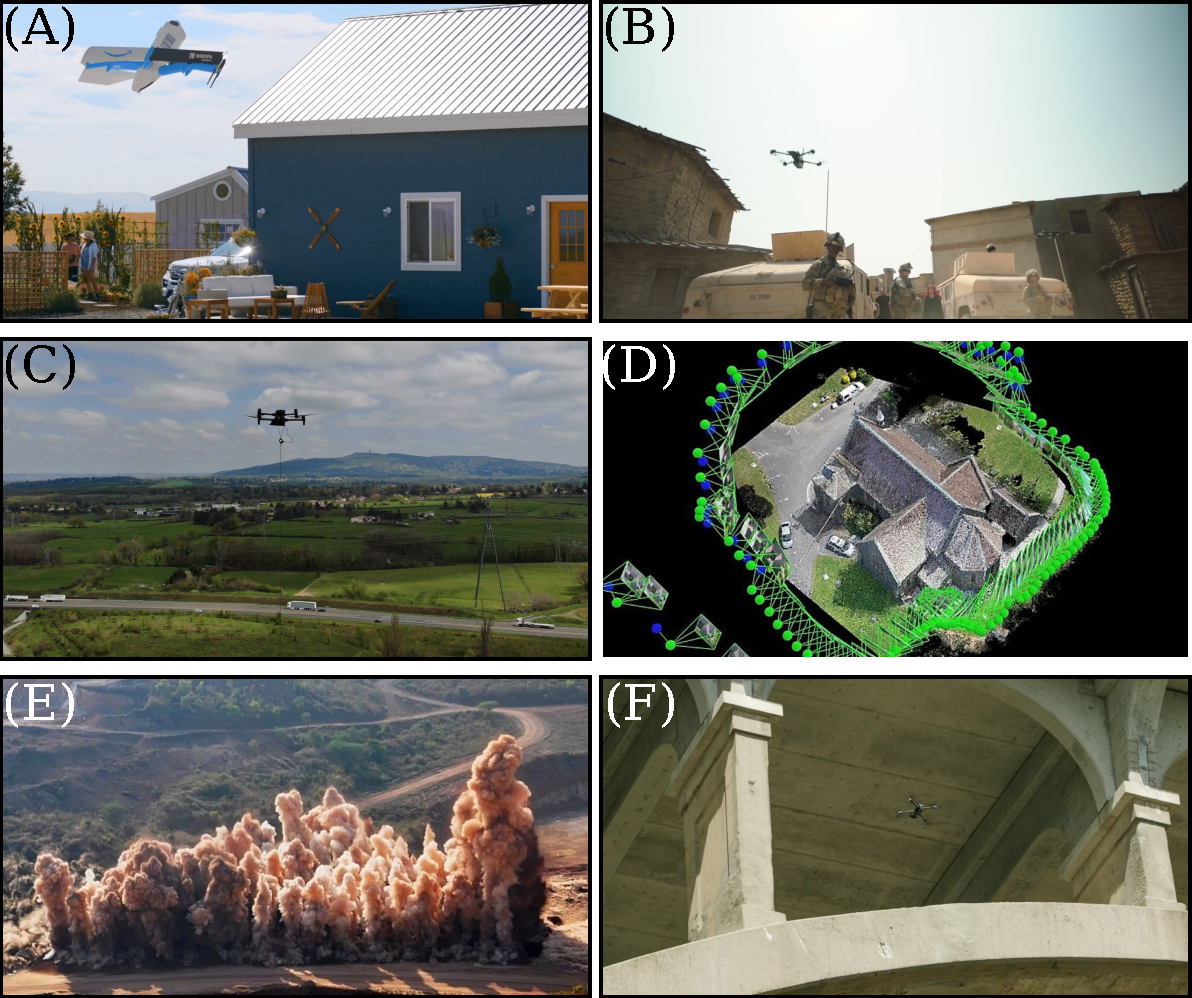
\includegraphics[width=\linewidth]{figs/misc/exAppsVertical.pdf}
                \captionsetup{labelformat=empty}
                \caption{\tiny{(A) \cite{amazonDelivery} (B) \cite{skydioMilitary} \\(C) \cite{trafficMonitor} (D) \cite{droneInspection} \\(E) \cite{propAero} (F) \cite{skydioInspection}}}
            \end{figure}
    \end{columns}
\end{frame}


\begin{frame}[t]{Example Transition Slide \hfill \includegraphics[height=.5cm]{figs/uncc/whiteUNCCLogo.eps}}
    \vspace{-0.4cm}
    \only<1>
    {
        \begin{figure}
            \centering
            \includegraphics[width=\linewidth]{figs/misc/speed1.pdf}
            % \caption{Categorical UAV top speed \cite{kakavitsasSurvey}}
            \captionsetup{labelformat=empty}
            \caption{\cite{kakavitsasSurvey}}
        \end{figure}
    }
    \only<2>{
        \begin{figure}
            \centering
            \includegraphics[width=\linewidth]{figs/misc/speed2.pdf}
            % \caption{Categorical UAV top speed \cite{kakavitsasSurvey}}
            \captionsetup{labelformat=empty}
            \caption{\cite{kakavitsasSurvey}}
        \end{figure}
    }
    \begin{columns}
        \column{0.7\textwidth}
            \vspace{-0.5cm}
            \only<1>{
                \begin{table}[h!]
                    \centering
                    \footnotesize{\begin{tabular}{p{2.2cm}p{2.2cm}p{2.2cm}}
                    \hline \hline
                     & Gust (mph) & Speed (mph) \\ \hline
                    Mean & 22 & 11.46 \\ 
                    Median & 21.3 & 10.8 \\ 
                    Max & 56.6 & 38.4 \\ \hline \hline
                    \end{tabular}}
                \end{table}
            }
            \only<2>{
                \begin{table}[h!]
                    \centering
                    \footnotesize{\begin{tabular}{p{2.2cm}p{2.2cm}p{2.2cm}}
                    \hline \hline
                     & Gust (mph) & Speed (mph) \\ \hline
                    Mean & 22 & 11.46 \\ 
                    Median & 21.3 & 10.8 \\ 
                    Max & \cellcolor[HTML]{ff9a82} 56.6 & \cellcolor[HTML]{ffff8e} 38.4 \\ \hline \hline
                    \end{tabular}}
                    % \scriptsize{\caption{Charlotte, NC windspeed and gust data for 2023 \cite{cltWind}}}
                \end{table}
            }
        \column{0.35\textwidth}
            % \begin{center}
            \small{Charlotte, NC wind speed and gust data for 2023-24 \cite{cltWind}}
            % \end{center}
    \end{columns}
    
\end{frame}

\begin{frame}{Thesis Statement \hfill \includegraphics[height=.5cm]{figs/uncc/whiteUNCCLogo.eps}}
    {Put your sample text here.  \emphPtGold{Emphasize points} with the commands defined in main.tex}
    \vspace{-0.2cm}
    Make a figure that defines all topics of your dissertation and ties in with the thesis statement at the top.
    \begin{figure}
        \centering
        \includegraphics[width=0.85\linewidth]{example-image-a}
    \end{figure}
\end{frame}

